\documentclass{beamer}

% imports and settings
%Deutsch
\usepackage[ngerman]{babel}
\usepackage[utf8]{inputenc}

%Mathematische Symbole
\usepackage{amsmath,amsfonts,amssymb}

%Halbtransparente Overlays
\setbeamercovered{transparent}

%Keine Navigation
\beamertemplatenavigationsymbolsempty

%Titelseite
\title{Programmiersprachen \& -paradigmen}
\subtitle{ein Überblick}
\author[Programmierpraktikum 2012]{Programmierpraktikum 2012}
\date{27.06.2012}

%Tags der PDF Datei
%TODO Tags%
\subject{}
\keywords{}

%Beamer Themes
\usetheme{Dresden}
\usecolortheme{orchid}
\usefonttheme{default}
\useinnertheme{default}
\useoutertheme{miniframes}

\setbeamertemplate{blocks}[rounded]

%Farbe
\usepackage{color}

%Java Listings
\usepackage{listings}
\lstloadlanguages{Java}

\lstset{language=Java,frame=single,captionpos=b,
	numbers=left,basicstyle=\tiny,breaklines=true,
	showstringspaces=false,
	keywordstyle=\color[rgb]{0.5,0,0.33},
	commentstyle=\color[rgb]{0.25,0.5,0.37},
	stringstyle=\color[rgb]{0.16,0,1}
}

%Latex Definitionen
\newcommand{\console}[1]{\begin{center}\colorbox{black}{\parbox{0.8\textwidth}{\textcolor{white}{#1}}}\end{center}}



\begin{document}
	\frame{
		\titlepage
	}
	\section{Übersicht}
	\subsection{}
	\frame{
		\frametitle{Übersicht}
		\begin{itemize}
			\item Eine kurze Geschichte des Programmierens
			\item Überblick Sprachen und Paradigmen
			\item Codegolf
			\item Esoterische Sprachen
		\end{itemize}
	}
	\section{Eine kurze Geschichte}
	\subsection{}
	\begin{frame}
		\frametitle{Jacquard-Webstuhl}
		\begin{columns}
			\begin{column}{5cm}
				\begin{overprint}
					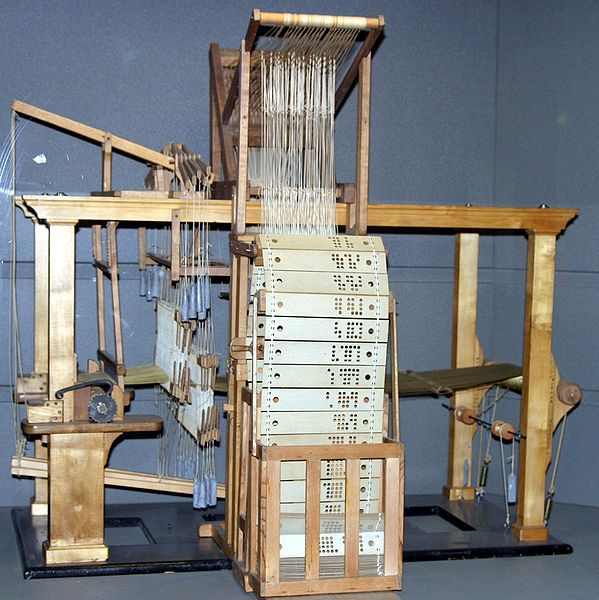
\includegraphics[width=45mm]{./images/webstuhl.jpg}
				\end{overprint}
			\end{column}
			\begin{column}{5cm}
				\begin{itemize}
				\item die erste programmierbare Maschine
				\item liest das zu webende Muster von Lochkarten
				\item und das 1805!
				\end{itemize}
			\end{column}
		\end{columns}
	\end{frame}
	\begin{frame}
		\frametitle{Der erste Bug}
		\begin{columns}
			\begin{column}{5cm}
				\begin{overprint}
					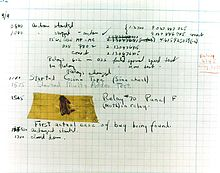
\includegraphics{./images/bug.jpg}
				\end{overprint}
			\end{column}
			\begin{column}{5cm}
				\begin{itemize}
				\item 1947 von Grace Hopper aus den Relais gezogen
				\item "First actual case of bug being found"
				\end{itemize}
			\end{column}
		\end{columns}
	\end{frame}
	\frame{
		\frametitle{Imperative Programmierung - Ausgangspunkt}
		\begin{itemize}
			\item Programm ist Folge von Befehlen
			\item Kontrollfluss durch Sprünge
			\item Beispiele: frühes Cobol / Algol / Fortran
			\item Und: Assembler!
			\item Gegensatz: Deklarative Programmierung - doch dazu später
		\end{itemize}
	}
	\frame{
		\frametitle{Strukturierte Programmierung}
		\begin{itemize}
			\item Erweiterung der imperativen Programmierung
			\item "Go To Statement Considered Harmful" \\- Edsger W. Dijkstra, 1968
			\item Kontrollstrukturen werden eingeführt
			\item Beispiele: Pascal, frühes Basic
		\end{itemize}
	}
	\frame{
		\frametitle{Prozedurale Programmierung}
		\begin{itemize}
			\item Erweiterung der strukturierten Programmierung
			\item Programme werden in Teilaufgaben / Prozeduren zerlegt
			\item wesentlicher Abstraktionsschritt ...
			\item ... in Richtung Hochsprache
			\item Beispiele: C, Pascal, Fortran, Algol, Cobol
		\end{itemize}
	}
	\frame{
		\frametitle{Modulare Programmierung}
		\begin{itemize}
			\item Erweiterung der prozeduralen Programmierung
			\item Programmteile werden in Module zusammengefasst
			\item Module enthalten Methoden und deren Daten
			\item Und das führt uns zur objektorientierten Programmierung
			\begin{itemize}
				\item Klassen statt Module
				\item Vererbung, Polymorphie, ....
				\item Beispiele: C++, Java, Python, und viele weitere
			\end{itemize}
		\end{itemize}
	}
	\frame{
		\frametitle{Und dann gab es da noch.....}
		\begin{itemize}
			\item komponentenorientiert
			\item aspektorientiert
			\item generativ
			\item generisch
			\item subjektorientiert
			\item datenstromorientiert
			\item konkatenativ
			\item und weitere, mehr oder weniger gruselige Namen
		\end{itemize}
	}
	\section{Sprachen und Paradigmen}
	\subsection{}
	\frame{
		\frametitle{Übersicht}
		\begin{itemize}
			\item In diesem Abschnitt "'interessantere"' Sprachen
			\item Und Beispiele dazu
			\item Wir werden uns ansehen:
			\begin{itemize}
				\item Python - Dynamische Sprache
				\item Haskell - Funktionale Sprache
				\item Prolog - Logische Sprache
			\end{itemize}
		\end{itemize}
	}
	\frame{
		\frametitle{Dynamisch?}
		\begin{itemize}
			\item Typisierung - Duck Typing
			\item Reflektion / Instrospektion
			\item late-binding
			\item häufig interpretiert \& mit Garbage Collection
		\end{itemize}
	}
	\frame{
		\frametitle{Duck Typing}
		
\includegraphics[width=90mm]{./images/ducktyping.jpg}
		\begin{center}
			"'When I see a bird that walks like a duck and swims like a duck and quacks 
			like a duck, I call that bird a duck."' \newline
			– James Whitcomb Riley
		\end{center}
	}
	\frame{
		\frametitle{Beispiele}
		\begin{center}
			Python Beispiele
		\end{center}
	}
	\frame{
		\frametitle{Einschub - Deklarative Programmierung}
		\begin{itemize}
			\item Beschreiben des Problems, nicht des Lösungswegs
			\item Finden der Lösung der Sprache überlassen
			\item Programme kürzer und leichter zu verstehen
			\item Bessere Beweisbarkeit
			\item in der Regel weniger performant
		\end{itemize}
	}
	\begin{frame}[containsverbatim]
		\frametitle{Deklarativ vs. Imperativ}
		\begin{center}
			\lstinputlisting[language={}]{./listings/quicksort-pascal.txt}
			\lstinputlisting[language={}]{./listings/quicksort-haskell.txt}
		\end{center}
	\end{frame}
	\frame{
		\frametitle{Funktional?}
		\begin{itemize}
			\item Programme bestehen aus Funktionen
			\begin{itemize}
				\item hängen nur von ihren Parametern ab
				\item haben keine Nebeneffekte
			\end{itemize}
			\item Funktionen höherer Ordnung
			\item Rekursive Funktionsaufrufe
		\end{itemize}
	}
	\frame{
		\frametitle{Auswertungsstrategie}
		\begin{itemize}
			\item strict - Argumente vor Funktionen
			\item eager - Ausdrücke als Ganzes
			\begin{itemize}
				\item lazy - Auswertung erst wenn nötig
				\item Ermöglicht unendliche Strukturen
			\end{itemize}
		\end{itemize}
	}
	\frame{
		\frametitle{Beispiele}
		\begin{center}
			Haskell Beispiele
		\end{center}
	}
		\frame{
		\frametitle{Logisch?}
		\begin{itemize}
			\item basierend auf mathematischer Logik
			\item Programm ist Menge von Axiomen und Folgerungen
			\item Interpreter versucht Anfrage zu "'beweisen"'
			\item Mehrere Lösungen für Anfrage möglich
		\end{itemize}
		}
	\frame{
		\frametitle{Beispiele}
		\begin{center}
			Prolog Beispiele
		\end{center}
	}
	\section{Codegolf und andere Späße}
	\subsection{}
	\frame{
		\frametitle{Codegolf - Mit welchem Schläger denn?}
		\begin{itemize}
			\item Unübliche Programmieraufgabe
			\item Unübliche Zielsetzung
			\item Teils extra Sprachen zum Codegolfen
			\item Beispiele sagen mehr als tausend Worte...
		\end{itemize}
	}
	\frame{
		\frametitle{We're no strangers to code golf, you know the rules, and so do I}
		\begin{itemize}
			\item Must output the lyrics exactly as they appear in the above pastebin. Here's the raw dump:
			 http://pastebin.com/raw.php?i=wwvdjvEj
			\item Cannot rely on any external resources - all lyrics must be generated by / embedded in code.
			\item No use of existing compression algorithms (e.g. gzip / bzip2) unless you include the full 
			algorithm in your code.
			\item Use any language, shortest code wins.
		\end{itemize}
	}
	\begin{frame}[fragile]
		\frametitle{Never gonna give up Ruby - 552 bytes}
		\begin{lstlisting}[language=Ruby]
			i=44
			s="We; n7trangMsL8loT63Ke rules5s8d8I
			AJull commit4nt'sChatFKink: of6CHldn'tRetKisJrom<ny@Ruy-/A= if?<sk 42DS'tLE 4?;Lo8bli=L7ee..
			O,R1)O,R001)/-.."
			"
			I justCannaLE?2Gotta >u=Msta=.|
			Ng1Nlet? downNrun<rH=5desMt?N>cryNsayRoodbyeNtE< lie5hurt?|
			
			We'T3n each@Jor s8lSg6r hear9<ch: but6;Lo7hyL7BInsideCe both3Cha9Ro: S
			We3KeRa45we;QplB|1)O)NgiT, nPgiT
			(G|iT? up| howFJeel:
			[...]
		\end{lstlisting}
		vollstädiger Code: http://codegolf.stackexchange.com/a/6166 by Ed. H.
	\end{frame}
	\frame{
		\frametitle{Anagramme}
		\begin{itemize}
			\item Eingabe: 2 Strings
			\item Erkenne ob Anagramm
			\item Wenigste Zeichen gewinnen
		\end{itemize}
	}
	\begin{frame}[fragile]
		\frametitle{Python - 32 byte}
		\begin{lstlisting}[language=Python]
			f=lambda a,b,S=sorted:S(a)==S(b)
		\end{lstlisting}
	\end{frame}
	\frame{
		\frametitle{Camelcase}
		\begin{itemize}
			\item Ich mag Tiere...
			\item ...oder ich bin aus dem Iran (Okay, Rassismuspunkt für mich)
			\item Ich möchte ein Programm, dass ein Kamel auf der Konsole ausgibt...
			\item ... dessen Sourcecode wie ein Kamel aussieht
		\end{itemize}
	}
	\begin{frame}[fragile]
			\frametitle{Camelcase}
			\tiny{
			\begin{lstlisting}[language=Perl, basicstyle=\tiny]
				#!/usr/bin/perl -w                                      # camel code
				use strict;
				
				                                           $_='ev
				                                       al("seek\040D
				           ATA,0,                  0;");foreach(1..3)
				       {<DATA>;}my               @camel1hump;my$camel;
				  my$Camel  ;while(             <DATA>){$_=sprintf("%-6
				9s",$_);my@dromedary           1=split(//);if(defined($
				_=<DATA>)){@camel1hum        p=split(//);}while(@dromeda
				 ry1){my$camel1hump=0      ;my$CAMEL=3;if(defined($_=shif
				        t(@dromedary1    ))&&/\S/){$camel1hump+=1<<$CAMEL;}
				       $CAMEL--;if(d   efined($_=shift(@dromedary1))&&/\S/){
				      $camel1hump+=1  <<$CAMEL;}$CAMEL--;if(defined($_=shift(
				     @camel1hump))&&/\S/){$camel1hump+=1<<$CAMEL;}$CAMEL--;if(
				     defined($_=shift(@camel1hump))&&/\S/){$camel1hump+=1<<$CAME
				     L;;}$camel.=(split(//,"\040..m`{/J\047\134}L^7FX"))[$camel1h
				      ump];}$camel.="\n";}@camel1hump=split(/\n/,$camel);foreach(@
				      camel1hump){chomp;$Camel=$_;y/LJF7\173\175`\047/\061\062\063\
				      064\065\066\067\070/;y/12345678/JL7F\175\173\047`/;$_=reverse;
				       print"$_\040$Camel\n";}foreach(@camel1hump){chomp;$Camel=$_;y
				        /LJF7\173\175`\047/12345678/;y/12345678/JL7F\175\173\0 47`/;
				         $_=reverse;print"\040$_$Camel\n";}';;s/\s*//g;;eval;   eval
				           ("seek\040DATA,0,0;");undef$/;$_=<DATA>;s/\s*//g;(   );;s
				             ;^.*_;;;map{eval"print\"$_\"";}/.{4}/g; __DATA__   \124
				               \1   50\145\040\165\163\145\040\157\1 46\040\1  41\0
				                    40\143\141  \155\145\1 54\040\1   51\155\  141
				                    \147\145\0  40\151\156 \040\141    \163\16 3\
				                     157\143\   151\141\16  4\151\1     57\156
				                     \040\167  \151\164\1   50\040\      120\1
				                     45\162\   154\040\15    1\163\      040\14
				                     1\040\1   64\162\1      41\144       \145\
				                     155\14    1\162\       153\04        0\157
				                      \146\     040\11     7\047\         122\1
				                      45\15      1\154\1  54\171          \040
				                      \046\         012\101\16            3\16
				                      3\15           7\143\15             1\14
				                      1\16            4\145\163           \054
				                     \040            \111\156\14         3\056
				                    \040\         125\163\145\14         4\040\
				                    167\1        51\164\1  50\0         40\160\
				                  145\162                              \155\151
				                \163\163                                \151\1
				              57\156\056
			\end{lstlisting}}
	\end{frame}
	\section{Esoterische Sprachen}
	\subsection{}
	\frame{
		\frametitle{Esoterische Sprachen - Motivation}
		\begin{itemize}
			\item nicht für den praktischen Einsatz gedacht
			\item ungewöhnliche Konzepte / Syntax
			\item Spaß
			\item ungewöhnliche Ziele
		\end{itemize}
	}
	\frame{
		\frametitle{Brainfuck}
		\begin{itemize}
			\item Ziele:
			\begin{itemize}
				\item touringmaschinenähnlich
				\item möglichst kleiner Compiler
			\end{itemize}
		\end{itemize}
	}
	\frame{
		\frametitle{Brainfuck - Befehle}
		\begin{itemize}
			\item \flq Zeiger inkrementieren
			\item \frq Zeiger dekrementieren
			\item + Wert inkrementieren
			\item - Wert dekrementieren
			\item . Wert als ASCII Zeichen ausgeben
			\item , Wert als ASCII Zeichen einlesen
			\item \lbrack Sprung nach vorne hinter passendes \rbrack
			\item \rbrack Sprung zurück wenn Wert ungleich Null
		\end{itemize}
	}
	\frame{
		\frametitle{Ook!}
		\begin{itemize}
			\item Brainfuck Dialekt mit leicht anderer Zielsetzung:
			\begin{enumerate}
				\item Eine Programmiersprache sollte schreib- und lesbar für Orang-Utans sein
				\item Die Syntax sollte einfach sein, leicht zu merken und das Wort Affe vermeiden
				\item Bananen sind gut!
			\end{enumerate}
			\item Es gibt drei Syntaxelemente, von denen jeweils zwei zu einem Ook-Tupel zusammengefasst werden
		\end{itemize}
	}
	\begin{frame}[containsverbatim]
		\frametitle{Brainfuck - Hello World}
		\begin{center}
			\lstinputlisting[language={}]{./listings/brainfuck-helloworld.txt}
		\end{center}
	\end{frame}
	\begin{frame}[containsverbatim]
		\frametitle{Ook - Hello World}
		\begin{center}
			\lstinputlisting[language={}]{./listings/ook-helloworld.txt}
		\end{center}
	\end{frame}
	\frame{
		\frametitle{Chef und SPL}
		\begin{itemize}
			\item Chef: Programmiersprache soll sich lesen wie ein Kochrezept
			\item Variablen = Zutaten, Stacks = Rührschüsseln, Befehle = mischen, rühren, backen...
			\item Shakespeare Programming Language: soll sich lesen wie ein Sonett
			\item ermöglichen sehr viel Freiheit bei der Ausgestaltung eines Programms
		\end{itemize}
	}
	\begin{frame}[containsverbatim]
		\frametitle{Chef - Hello World}
		\begin{center}
			\lstinputlisting[language={}]{./listings/chef-helloworld.txt}
		\end{center}
	\end{frame}
	\frame{
		\frametitle{Malbolge}
		\begin{itemize}
			\item Ziel: Schlimmstmögliche Programmiersprache
			\item Verwendet den ASCII Wert eines Zeichens als Befehl
			\item - Effekt eines Befehls hängt von Speicherstelle ab (modulo 94)
			\item - und plus einen Zähler (auch auf Datenpointer)
			\item - Speicherzugriffe nur ternär
			\item - nur unconditional jumps
			\item So kompliziert, dass das erste lauffähige Malbolge Programm von einem Suchalgorithmus gefunden wurde......
		\end{itemize}
	}
	\begin{frame}[containsverbatim]
		\frametitle{Malbolge - Hello World}
		\begin{center}
			\lstinputlisting[language={}]{./listings/malbolge-helloworld.txt}
		\end{center}
	\end{frame}
	\section{Beispiele, Fragen, Abschluss}
	\subsection{}
	\frame{
		\frametitle{Noch Fragen?}
		\begin{center}
			{\bf \Large Gibt es noch Fragen oder Unklarheiten?}
		\end{center}
	}
	\frame{
		\frametitle{Dann bleibt nur noch...}
		\begin{center}
			{\bf \Large Vielen Dank für Ihre Aufmerksamkeit!}
		\end{center}
	}
\end{document}
